\documentclass{article}

\usepackage{amsmath, amsthm, amssymb, amsfonts}
\usepackage{thmtools}
\usepackage{graphicx}
\usepackage{setspace}
\usepackage{geometry}
\usepackage{float}
\usepackage{hyperref}
\usepackage[utf8]{inputenc}
\usepackage[english]{babel}
\usepackage{framed}
\usepackage[dvipsnames]{xcolor}
\usepackage{tcolorbox}

%Define the listing package
\usepackage{listings} %code highlighter
\usepackage{color} %use color
\definecolor{mygreen}{rgb}{0,0.6,0}
\definecolor{mygray}{rgb}{0.5,0.5,0.5}
\definecolor{mymauve}{rgb}{0.58,0,0.82}
 
%Customize a bit the look
\lstset{ %
backgroundcolor=\color{white}, % choose the background color; you must add \usepackage{color} or \usepackage{xcolor}
basicstyle=\footnotesize, % the size of the fonts that are used for the code
breakatwhitespace=false, % sets if automatic breaks should only happen at whitespace
breaklines=true, % sets automatic line breaking
captionpos=b, % sets the caption-position to bottom
commentstyle=\color{mygreen}, % comment style
deletekeywords={...}, % if you want to delete keywords from the given language
escapeinside={\%*}{*)}, % if you want to add LaTeX within your code
extendedchars=true, % lets you use non-ASCII characters; for 8-bits encodings only, does not work with UTF-8
frame=single, % adds a frame around the code
keepspaces=true, % keeps spaces in text, useful for keeping indentation of code (possibly needs columns=flexible)
keywordstyle=\color{blue}, % keyword style
% language=Octave, % the language of the code
morekeywords={*,...}, % if you want to add more keywords to the set
numbers=left, % where to put the line-numbers; possible values are (none, left, right)
numbersep=5pt, % how far the line-numbers are from the code
numberstyle=\tiny\color{mygray}, % the style that is used for the line-numbers
rulecolor=\color{black}, % if not set, the frame-color may be changed on line-breaks within not-black text (e.g. comments (green here))
showspaces=false, % show spaces everywhere adding particular underscores; it overrides 'showstringspaces'
showstringspaces=false, % underline spaces within strings only
showtabs=false, % show tabs within strings adding particular underscores
stepnumber=1, % the step between two line-numbers. If it's 1, each line will be numbered
stringstyle=\color{mymauve}, % string literal style
tabsize=2, % sets default tabsize to 2 spaces
title=\lstname % show the filename of files included with \lstinputlisting; also try caption instead of title
}
%END of listing package%
 
\definecolor{darkgray}{rgb}{.4,.4,.4}
\definecolor{purple}{rgb}{0.65, 0.12, 0.82}
 
%define Javascript language
\lstdefinelanguage{JavaScript}{
keywords={typeof, new, true, false, catch, function, return, null, catch, switch, var, if, in, while, do, else, case, break},
keywordstyle=\color{blue}\bfseries,
ndkeywords={class, export, boolean, throw, implements, import, this},
ndkeywordstyle=\color{darkgray}\bfseries,
identifierstyle=\color{black},
sensitive=false,
comment=[l]{//},
morecomment=[s]{/*}{*/},
commentstyle=\color{purple}\ttfamily,
stringstyle=\color{red}\ttfamily,
morestring=[b]',
morestring=[b]"
}
 
\lstset{
language=JavaScript,
extendedchars=true,
basicstyle=\footnotesize\ttfamily,
showstringspaces=false,
showspaces=false,
numbers=left,
numberstyle=\footnotesize,
numbersep=9pt,
tabsize=2,
breaklines=true,
showtabs=false,
captionpos=b
}

\colorlet{LightGray}{White!90!Periwinkle}
\colorlet{LightOrange}{Orange!15}
\colorlet{LightGreen}{Green!15}

\newcommand{\HRule}[1]{\rule{\linewidth}{#1}}

\NewEnviron{NORMAL}{% 
    \scalebox{2}{$\BODY$} 
} 

\declaretheoremstyle[name=Theorem,]{thmsty}
\declaretheorem[style=thmsty,numberwithin=section]{theorem}
\tcolorboxenvironment{theorem}{colback=LightGray}

\declaretheoremstyle[name=Proposition,]{prosty}
\declaretheorem[style=prosty,numberlike=theorem]{proposition}
\tcolorboxenvironment{proposition}{colback=LightOrange}

\declaretheoremstyle[name=Principle,]{prcpsty}
\declaretheorem[style=prcpsty,numberlike=theorem]{principle}
\tcolorboxenvironment{principle}{colback=LightGreen}

\setstretch{1.2}
\geometry{
    textheight=9in,
    textwidth=5.5in,
    top=1in,
    headheight=12pt,
    headsep=25pt,
    footskip=30pt
}

% ------------------------------------------------------------------------------

\begin{document}

% ------------------------------------------------------------------------------
% Cover Page and ToC
% ------------------------------------------------------------------------------

\title{ \normalsize \textsc{}
		\\ [2.0cm]
		\HRule{1.5pt} \\
		\LARGE \textbf{\uppercase{Calcolo Numerico}
		\HRule{2.0pt} \\ [0.6cm] \LARGE{Corso A} \vspace*{10\baselineskip}}
		}
        
\date{\text{Ultima Compilazione - }\today}
\author{\textbf{Autore} \\ 
		Giuseppe Acocella \\
		2024/25\\
        \url{https://github.com/Peenguino}}

\maketitle
\newpage

\tableofcontents

\newpage

%\begin{figure}[htbp]
    %\center
    %\includegraphics[scale=0.4]{img/classiComplessita2.png}
%\end{figure}

\section{Introduzione}

I temi principali trattati in questi appunti saranno riguardanti i processi matematici che ci permettono di analizzare la conversione da continuo a discreto, per poter fornire questi dati ad una macchina finita. Spesso questi approcci vengono utilizzati anche quando la complessità di un determinato algoritmo è troppo elevata e di conseguenza si preferisce analizzare delle approssimazioni discrete.

\vspace*{15px}

\subsection{Fasi dell'Analisi Numerica}

Elenchiamo le fasi dell'Analisi Numerica:

\begin{enumerate}
    \item La prima fase è lo studio del \textbf{Mondo Reale} che osserviamo.
    \item Grazie all'osservazione del \textbf{Mondo Reale} generiamo un \textbf{Modello Matematico Continuo} in una seconda fase.
    \item La terza fase cerca di \textbf{discretizzare} il modello precedente in uno \textbf{discreto}. Questo genera un errore detto \textbf{errore analitico}.
    \item Si cerca un \textbf{Metodo di Risoluzione} al \textbf{Modello Matematico Discreto} durante una quarta fase. Questo genera un errore detto \textbf{errore inerente}, dato dalla rappresentazione discreta di qualcosa di continuo.
    \item L'ultima fase è quella della \textbf{Soluzione Approssimata} trovata dal 
    \newline \textbf{Metodo di Risoluzione} proposto. Questo produce un errore detto \textbf{errore algoritmico}.
\end{enumerate}

\vspace*{15px}

\subsection{Errore Inerente ed Errore di Approssimazione}

Consideriamo una $x$ continua, la sua rappresentazione su una macchina sarà $\overline{x}$. Definiamo dunque i due errori $\varepsilon_{IN}$ ed $\varepsilon_{x}$:

\vspace*{8px}

\begin{enumerate}
    \item \textbf{Errore Inerente} $(\varepsilon_{IN})$: Assumendo una funzione $f$:
    \[ \varepsilon_{IN} \: = \frac{f(\overline{x}) \: - \: f(x)}{f(x)} \]

\vspace*{8px}

    \item \textbf{Errore di Approssimazione} $(\varepsilon_{x})$: Assumendo una funzione $f$:
    \[ \varepsilon_{x} \: = \frac{\overline{x} \: - \: x}{x} \]
\end{enumerate}

\newpage

\subsection{Rappresentazione Virgola Fissa vs Virgola Mobile}

Immaginiamo di avere una quantità $k$ fissata di bit da poter utilizzare per rappresentare un numero su una macchina. Descriviamo due potenziali metodologie di rappresentazione:

\begin{enumerate}
    \item \textbf{Numeri a virgola fissa}: Si compongono di un \textbf{segno}, una \textbf{parte intera} ed una \textbf{parte frazionaria}.
    \item \textbf{Numeri a virgola mobile}: Si compongono di una \textbf{mantissa} ossia un numero compreso tra $0$ ed $1$ (estremi esclusi), un \textbf{segno} ed un \textbf{esponente}.
\end{enumerate}

\subsection{Teorema di Rappresentazione in Base}

Sia $x \in \mathbb{R}$, $x \neq 0$, allora scelta una base $\beta$ di rappresentazione \textbf{esistono} e \textbf{sono unici}:

\begin{enumerate}
    \item Un valore $\rho \in \mathbb{Z}$ detto \textbf{esponente}.
    \item Una successione $ \{ d_{i} \}_{i=1,2...}$ dette \textbf{cifre}.
    \item $d_{i}$ non tutte uguali a $\beta -1$ da un certo punto in poi.
\end{enumerate}

tali che:

\[ x \: = \: segno(x) \: \beta^{\rho} \: (\sum^{\infty}_{i=1} d_{i}\beta^{-i} ) \]

\subsubsection{Motivazioni e commenti}

\begin{enumerate}
    \item $d\neq0$ altrimenti avrei \textbf{rappresentazioni diverse} di \textbf{stessi numeri}, di conseguenza cadrebbe l'\textbf{unicità} delle rappresentazioni.
    \item $d_{i}$ non tutte uguali a $\beta -1$ da un certo punto in poi altrimenti numeri come $0.\overline{9}$ convergerebbe ad $1$.
\end{enumerate}

\vspace*{10px}

\subsection{Insieme di Numeri di Macchina}

Definiamo l'insieme $\Phi$ che permette la rappresentazione dei numeri di macchina:

\[ \Phi(\beta, t, m,M) = \: \{0\} \: \cup \: \{ x \in \mathbb{R} \: , x \: = \: segno(x) \: \beta^{\rho} \: (\sum^{t}_{i=1} d_{i}\beta^{-i} ) \} \]

\begin{enumerate}
    \item $\beta$: \textbf{base}.
    \item $t$ cifre della \textbf{mantissa}.
    \item $-n\leq \rho \leq M$, ossia i due \textbf{estremi} che contengono l'\textbf{esponente} $\rho$.
    \item Sono necessarie delle ipotesi a supporto dell'\textbf{unicità} di questa formulazione:
    \begin{enumerate}
        \item $0 \leq d_{i} \leq \beta-1$
        \item $d_{1} \neq 0$
    \end{enumerate}
\end{enumerate}

\newpage

\subsubsection{Cardinalità dell'Insieme di Numeri di Macchina}

\[ \# \Phi (\beta, t, m,M) = 1 \: + \: 2 (n+M+1)(\beta-1)(\beta^{t-1}) \]

\begin{enumerate}
    \item $1$ è la cardinalità dello \textbf{zero}.
    \item Il prodotto con $2$ è dato dal \textbf{segno}.
    \item $(n+M+1)$ tutte le possibili \textbf{configurazioni} dell'\textbf{esponente} $\rho$.
    \item $(\beta-1)$ tutte le possibili \textbf{configurazioni} delle \textbf{cifre} rispetto alla base (escluso lo zero).
    \item $(\beta^{t-1})$ avendo $t$ \textbf{bit disponibili} e $\beta$ la \textbf{base}, allora ho tutte le possibili \textbf{combinazioni} (escluse tutte quelle che iniziano con lo zero).
\end{enumerate}

\subsubsection{Numero più piccolo/più grande}

Analizziamo la rappresentazione del numero $\omega$ \textbf{più piccolo} e del numero $\Omega$ più grande.

\begin{enumerate}
    \item Numero \textbf{più piccolo} rappresentabile $\omega$:
    \[ \omega = \beta^{-m}(0.10...0)_{\beta} = (\beta^{-m})(\beta^{-1}) = \beta^{-m-1} \]
Questo perchè vogliamo la nostra base $\beta$ elevata al più piccolo estremo degli esponenti $-m$ moltiplicata alla più piccola mantissa nella base corrente.
    \item Numero \textbf{più grande} rappresentabile $\Omega$:
    \[ \Omega = \beta^{M}(0.[\beta-1][\beta-1][\beta-1]) = \beta^{M}(1-\beta^{-t}) \]
Questo perchè vogliamo la \textbf{base} $\beta$ elevata al più grande dei possibili esponenti $M$, ripetendo nella mantissa tutte le cifre più grandi permesse dalla base.
    
\end{enumerate}

\vspace*{10px}

\subsubsection{Standard IEEE}

Lo \textbf{Standard IEEE} può essere rappresentato come istanza di $\Phi$:

\[ Standard_{IEEE}\:=\:\Phi(2,53,1021,1024) \]

Contando $1$ bit per il segno e $11$ bit per l'esponente, $52$ bit vengono dedicati alla mantissa ed ad alcuni simboli speciali, come $NaN$ oppure $\infty$.

\vspace*{10px}

\paragraph{Underflow/Overflow} Una volta stabilito questo standard, se l'esponente $\rho$ esce \newline dall'intervallo $[-m,M]$, allora:

\begin{enumerate}
    \item Se $\rho > M$ allora è \textbf{overflow}, e ad esempio in Matlab questo comportamento viene approssimato ad $\infty$.
    \item Se $\rho < -m$ allora è \textbf{underflow}, e in Matlab questo comportamento viene approssimato a $0$.
\end{enumerate}

\newpage

\section{Studio dell'Errore}

\subsection{Troncamento/Arrotondamento}

Se $\rho \in [-m,M]$ allora possono succedere due cose:

\begin{enumerate}
    \item $x \in \mathbb{R}$ si rappresenta su $t$ cifre della mantissa disponibili.
    \item $x \in \mathbb{R}$ ha bisogno di più cifre rispetto a quelle fornite per la mantissa. In questo caso posso operare in due modi:
    \begin{enumerate}
        \item \textbf{Troncamento}: $x$ viene rappresentato con il numero di macchina subito prima. Quindi $x$ viene rappresentato con il numero di macchina $\tilde{x}$ che sia più grande rappresentabile con $|\tilde{x} |\leq |x|$.
        \item \textbf{Arrotondamento}: $x$ viene rappresentato con $\tilde{x}$ numero di macchina più vicino.
    \end{enumerate}
\end{enumerate}

\paragraph{Errore Assoluto/Relativo}

Definiamo due tipi di errore:

\begin{enumerate}
    \item \textbf{Errore Assoluto} $(\epsilon)$:
    \[ \epsilon = \tilde{x} - x \]
    \item \textbf{Errore Relativo} $(\epsilon_{x})$:
    \[ \epsilon_{x} = \frac{\tilde{x} - x}{x} \]
    
\end{enumerate}

\subsubsection{Teorema di Errore di Rappresentazione (con Dim.)}

Sia $x \in \mathbb{R}$, $x \neq 0$ e $\omega \leq |x| \leq \Omega$ allora:

\begin{enumerate}
    \item Identificando con $u$ la \textbf{precisione di macchina}:
    \[ |\epsilon_{x}| < u \]
    ed oltre a questo:
    \begin{enumerate}
        \item Operando con \textbf{troncamento}:
        \[ u \: = \: \beta^{1-t} \]
        \item Operando con \textbf{arrotondamento}:
        \[ u \: = \: \frac{1}{2}\beta^{1-t} \]
    \end{enumerate}
\end{enumerate}

\newpage

\paragraph{Dimostrazione}

\begin{enumerate}
    \item Rappresentazione in base: 
    \[ x \: = \: \beta^{\rho} \: (\sum^{\infty}_{i=1} d_{i}\beta^{-i}) \:\:\: \text{con} \:\:\: \rho \in [-m,M] \]
    \item Assumiamo di star considerando i numeri di macchina in troncamento, dunque cambia l'indice della sommatoria in $t$ cifre:
    \[ x \: = \: \beta^{\rho} \: (\sum^{t}_{i=1} d_{i}\beta^{-i}) \:\:\: \text{con} \:\:\: \rho \in [-m,M] \]
    \item ****
    \[ |\tilde{x} - x| < |b-a| \]
    \item ***
    \[ |x| \geq \beta^{\rho-1} \: = \: \beta^{\rho}(0.1)_{\beta} \]
    \item Dunque alla fine possiamo ricavare $\tilde{x}$ della nostra macchina:
    \[ \boxed{\tilde{x} \: = \: x(1+\epsilon_{x})} \]
\end{enumerate}

\newpage

\subsection{Operazioni di Macchina}

Assumendo $\tilde{x},\tilde{y}$ con $\tilde{x},\tilde{y} \in \Phi(10,t,5,5)$ ma con $\tilde{x}+\tilde{y} \notin \Phi(10,t,5,5)$, risulta necessario definire nuove operazioni, ossia delle \textbf{operazioni di macchina}:
\begin{enumerate}
    \item \textbf{Operazione Somma}: Prendiamo la versione in floating point dell'operazione somma originale:
        \[\tilde{x} \oplus \tilde{y} = fl(\tilde{x}+\tilde{y})\]
    e l'\textbf{errore} generato sarà:
    \vspace*{10px}
    \[ \epsilon = \frac{(\tilde{x} \oplus \tilde{y}) - (\tilde{x} + \tilde{y})}{(\tilde{x} + \tilde{y})} \]
    \vspace*{10px}
    Si associa quindi un operazione reale ad una approssimativa di macchina, quindi anche che
    \[ |\epsilon| < u \]
    \item \textbf{Operazione Differenza}: Allo stesso modo approcciamo la differenza, anch'essa produrrà un errore:
    \vspace*{10px}
    \[ \epsilon = \frac{(\tilde{x} \oplus \tilde{y}) - (x + y)}{(x + y)} \]
    \vspace*{10px}
\end{enumerate}

\subsubsection{Errore nella Somma e suo Relativo Ordine (con Dim.)}

Mostriamo per step questa dimostrazione:

\begin{enumerate}
    \item Definizione di $\tilde{x}$:
    \[ {\tilde{x} \: = \: x(1+\epsilon_{x})} \:\:\:,\:\:\: {\tilde{y} \: = \: y(1+\epsilon_{y})}\]
    \item Prendiamo in considerazione \textbf{solo} l'errore sull'\textbf{operazione somma}:
    \[ \tilde{x} \oplus \tilde{y} = (\tilde{x} + \tilde{y})(1+\epsilon)\]
    \item Sostituiamo le definizioni di $(1.)$ in $(2.)$:
    \[ \tilde{x} \oplus \tilde{y} = [x(1+\epsilon_{x}) + y(1+\epsilon_{y})](1+\epsilon) \]
    \newpage
    \item Svolgiamo i prodotti:
    \[ \tilde{x} \oplus \tilde{y} = (x+y) + x\epsilon_{x} + y\epsilon_{y} + (x+y)\epsilon + x\epsilon_{x}\epsilon + y\epsilon_{y}\epsilon \]
    \item Considerando il fatto che gli ultimi due operandi sono generati dal prodotto di due epsilon diversi, li ignoriamo effettuando un \textbf{approssimazione al prim'ordine}:
    \[ \tilde{x} \oplus \tilde{y} = (x+y) + x\epsilon_{x} + y\epsilon_{y} + (x+y)\epsilon \]
    \item Tornando alla definizione di $\epsilon_{TOT}$ dell'operazione somma:
    \[ \epsilon = \frac{(\tilde{x} \oplus \tilde{y}) - (x + y)}{(x + y)} \]
    \vspace*{10px}
    Effettuiamo sostituzione di $\tilde{x} \oplus \tilde{y}$ approssimati al prim'ordine:
    \[ \epsilon_{TOT} = \frac{[(x+y) + x\epsilon_{x} + y\epsilon_{y} + (x+y)\epsilon] - (x + y)}{(x + y)} \: = \]
    \[ = \frac{x}{x+y}\epsilon_{x} + \frac{y}{x+y}\epsilon_{y} + \epsilon \]
    \item Otteniamo dunque i primi due operandi che rappresentano l'\textbf{errore inerente}, ossia quello che si propaga dalle precedenti operazioni, e l'\textbf{errore algoritmico}, causato dalla corrente operazione:
    \[ \boxed{\epsilon_{TOT} = \frac{x}{x+y}\epsilon_{x} + \frac{y}{x+y}\epsilon_{y} + \epsilon} \]
    \item Rendendo generica la formula ottenuta definiamo dei \textbf{coefficienti di amplificazione}:
    \[ \boxed{ \epsilon_{TOT} = \epsilon_{OP} + C_{1}\epsilon_{TOT}^{(k)} + C_{2}\epsilon_{TOT}^{(s)} } \]
    Questa formula di $\epsilon_{TOT}$ si basa su una generica operazione
    \[ \boxed{z^{(i)} = z^{(k)} \: op \:z^{(k)}} \]
    
\end{enumerate}

\newpage

\subsubsection{Teorema di Errore di Calcolo Funzione Razionale (con Dim.)}

Calcolo dell'errore totale $\epsilon_{TOT}$:

\[ \boxed{\epsilon_{TOT} = \epsilon_{IN} + \epsilon_{ALG}} \]

dove:

\begin{enumerate}
    \item L'\textbf{Errore Inerente} dipende esclusivamente dal problema:
    \[ \boxed{\epsilon_{IN} = \frac{f(\tilde{x}) - f(x)}{f(x)}} \]
    \item L'\textbf{Errore Algoritmico} dipende dalla scelta della funzione scelta:
    \[ \boxed{\epsilon_{ALG} = \frac{g(\tilde{x}) - f(\tilde{x})}{f(x)}} \]
\end{enumerate}

\paragraph{Dimostrazione}

\begin{enumerate}
    \item Prendendo $\epsilon_{TOT}$ (inteso come somma di $\epsilon_{IN}$ e $\epsilon_{ALG}$) sommiamo e sottraiamo $f(\tilde{x})$:
    \[ \epsilon_{TOT} = \epsilon_{IN} + \epsilon_{ALG} =\]
    \[ = \: \frac{g(\tilde{x})-f(x)+f(\tilde{x})-f(\tilde{x})}{f(x)} \]
    \item Distribuisco in modo tale da poter ricavare l'\textbf{errore inerente} (secondo operando):
    \[ \epsilon_{TOT} = \frac{g(\tilde{x})-f(\tilde{x})}{f(x)} \: + \: \frac{f(\tilde{x})-f(x)}{f(x)}  \]
    \item Moltiplico e divido per $f(\tilde{x})$ e scambio tra loro i due denominatori:
    \[ \epsilon_{TOT} = \frac{g(\tilde{x})-f(\tilde{x})}{f(\tilde{x})} \: * \: \frac{f(\tilde{x})}{f(x)}\:+\:\epsilon_{IN}  \]
    \item Notiamo che il primo fattore del primo operando corrisponde all'errore algoritmico:
    \[ \epsilon_{TOT} = \epsilon_{ALG} \: * \: \frac{f(\tilde{x})}{f(x)}\:+\:\epsilon_{IN}  \]
    \item Assumendo che $\epsilon_{IN+1} = \frac{f(\tilde{x})}{f(x)}$ sostituiamo:
    \[ \epsilon_{TOT} = (\epsilon_{ALG})(\epsilon_{IN+1})\:+\:\epsilon_{IN}  \]
    \item Approssimiamo $\epsilon_{ALG} \doteq (\epsilon_{ALG})(\epsilon_{IN+1})$:
    \[ \boxed{\epsilon_{TOT} = \epsilon_{IN} + \epsilon_{ALG}} \]
    
\end{enumerate}

\newpage

\subsubsection{Condizionamento vs Stabilità}

Descriviamo le differenze tra \textbf{condizionamento} e \textbf{stabilità}:

\begin{enumerate}
    \item \textbf{Condizionamento}: Studio dell'errore, errore intrinseco.
    \item \textbf{Stabilità}: Studio dell'errore algoritmico, rappresenta la stabilità
    \newline
    numerica dell'algoritmo proposto.
\end{enumerate}

\subsubsection{Teorema Coefficiente di Amplificazione ed Errore Inerente (con Dim.)}

Sia $f(x) \in C^{2}$ (ossia derivabili due volte con entrambe le derivate continue), allora:

\[ \boxed{\epsilon_{IN} = \frac{x}{f(x)}f^{'}(x)\epsilon_{x}} \]

Grazie a questo possiamo determinare se un problema risulta mal condizionato o ben condizionato:

\begin{center}
    \begin{tabular}{ c | c | c | c | c }
    & somma & sottrazione & prodotto & divisione \\
    \hline
    c1 & $\frac{x}{x+y}$ & $\frac{x}{x-y}$ & $1$ & $1$ \\
    \hline
    c2 & $\frac{y}{x+y}$ & $\frac{-y}{x-y}$ & $1$ & $-1$ \\
    \hline
    \end{tabular}
\end{center}

\vspace*{5px}

\begin{enumerate}
    \item \textbf{Ben Condizionato}: Non ho punti nel dominio del coefficiente di amplificazione dove la funzione va a $\infty$.
    \item \textbf{Mal Condizionato}: Ho dei punti in cui il coefficiente può andare a $\infty$. Dunque un problema può essere mal condizionato in specifici intervalli.
\end{enumerate}

\paragraph{Dimostrazione}

\begin{enumerate}
    \item Riprendiamo lo sviluppo di Taylor fino al secondo ordine:
    \[ f(x) = f(x_0) + f^{'}(x_0)(x-x_0) + f^{''}(x_0)\frac{(x-x_0)^{2}}{2!}\]
    \vspace*{8px}
    \item Contestualizziamo ad $\tilde{x}$:
    \[ f(\tilde{x}) = f(x) + f^{'}(x)(\tilde{x}-x) + f^{''}(x)\frac{(\tilde{x}-x)^{2}}{2!}\]
    \vspace*{8px}
    \item Porto a sinistra $f(x)$:
    \[ f(\tilde{x}) -f(x) = f^{'}(x)(\tilde{x}-x) + f^{''}(x)\frac{(\tilde{x}-x)^{2}}{2!}\]
    \newpage
    \item Moltiplico e divido per $x$ il primo operando a sinistra e moltiplico e divido per $x^{2}$ il secondo operando a sinistra:
    \[ f(\tilde{x}) -f(x) = xf^{'}(x)\frac{(\tilde{x}-x)}{x} + x^{2}\frac{f^{''}(x)\frac{(\tilde{x}-x)^{2}}{2!}}{x^{2}}\]
    \item Considerando che:
    \begin{enumerate}
        \item Errore $\epsilon_{x}$ ed $\epsilon^{2}_{x}$:
        \vspace*{5px}
        \[ \boxed{\epsilon_{x} = \frac{(\tilde{x}-x)}{x}} \:\:\: \boxed{\epsilon^{2}_{x} = \frac{(\tilde{x}-x)^{2}}{x^2}} \]
    \end{enumerate}
    \vspace*{8px}
    \item Sostituiamo con $\epsilon_{x}$ ed approssimiamo al prim'ordine ignorando $\epsilon^{2}_{x}$:
    \[ f(\tilde{x}) - f(x) = xf^{'}(x)\epsilon_{x} \]
    \vspace*{8px}
    \item Dunque infine otteniamo la formula generica:
    \[ \boxed{\epsilon_{IN} = \sum_{i=1}^{n} \frac{x_{i}}{f(x_{1},...,x_{n})} \frac{\delta f}{\delta x_{i}} \epsilon_{x_{i}}} \]
\end{enumerate}

\vspace*{15px}

\subsubsection{Errore di Calcolo Funzione Irrazionale}

Assumiamo di voler rappresentare in macchina $e^x$. E' necessario trovare una funzione che approssimi la funzione irrazionale $e^x$:

\begin{enumerate}
    \item Definiamo $e^x$ ed $EXP(x)$:
    \[ \boxed{e^{x} = \sum^{\infty}_{i=0} \frac{x^{i}}{i!}} \: \: \: \: \: \: \: \: \boxed{EXP(x) = \sum^{n}_{i=0} \frac{x^{i}}{i!}} \]
    \item Valutiamo quanto intercorre tra le due con l'errore di \textbf{Lagrange}:
    \[ e^x = EXP(x) + \frac{\epsilon^{(n+1)}_{x}}{(n+1)!} \]
\end{enumerate}

In questo modo abbiamo stabilito che errore viene effettuato approssimando $e^x$ con $EXP(x)$.

\newpage

\section{Algebra Lineare Numerica - Computazione e Condizionamento}

Questo capitolo analizzerà strumenti base dell'algebra lineare che successivamente saranno richiesti per problemi su spazi vettoriali.

\subsection{Norme Vettoriali}

La norma è una \textbf{funzione} che ci permette di ricavare un informazione quantitativa dato un oggetto di uno specifico spazio vettoriale.

\paragraph{Definizione} Sia $f: F^{n} \xrightarrow{} \mathbb{R}$ tale che:

\begin{enumerate}
    \item $f(x) \geq 0 $ e $f(x) = 0$ se e solo se $x = \begin{bmatrix}
0 \\
. \\
. \\
0
\end{bmatrix}$

    \item $f(\alpha x) \: = \: |\alpha|f(x) \: \: \: \forall \alpha \in F $
    \item $f(x+y) \leq f(x) + f(y)$
\end{enumerate}

Allora $f$ è una norma vettoriale su $F$ e si definisce con $\boxed{|| \:\:\:||}$

\subsubsection{Distanza, Norma 1, Norma 2, Norma Infinito}

Elenchiamo queste definizioni:

\begin{enumerate}
    \item \textbf{Distanza}:
    \[ d(x,y) = || \: x - y \:|| \]
    \item \textbf{Norma 1}:
    \vspace*{12px}
    \[ \boxed{|| x ||_{1} = \sqrt{\sum^{n}_{i=1}}|x_{i}|} \]
    \vspace*{4px}
    \item \textbf{Norma 2}:
    \vspace*{12px}
    \[ \boxed{|| x ||_{2} = \sqrt{\sum^{n}_{i=1}}|x_{i}|^2} \]
    \vspace*{4px}
    \item \textbf{Norma Inf*}:
    \vspace*{12px}
    \[ \boxed{|| x ||_{\infty} = max|x|} \]
    \vspace*{4px}
\end{enumerate}

\newpage

\paragraph{Equivalenza Topologica} Date due norme $||\:||_{(1)}$ e $||\:||_{(2)}$ allora $\exists \: \alpha,\beta \in F$ tale che $\forall \: v \in F^{n}$:
\[ \alpha||v||_{(2)} \leq ||v|| \leq \beta||v||_{(1)}\]

Da questo posso ottenere informazioni riguardo divergenza e convergenza se utilizzato "simil th. dei carabinieri".

\subsection{Norma Matriciale}

Contestualizziamo la norma alle matrici:

\paragraph{Definizione} Sia $f: F^{nxn} \xrightarrow{} \mathbb{R}$ tale che:

\begin{enumerate}
    \item $f(A) \geq 0$ e $f(A) = 0$ se e solo se $A = [0]_{nxn}$
    \item $f(\alpha A) = |\alpha|f(A)$
    \item $f(A+B) = f(A) + f(B)$
    \item $f(AB) \leq f(A)f(B)$
\end{enumerate}

\subsubsection{Norma Matriciale indotta da Norma Vettoriale}

\vspace*{10px}

\[ \boxed{||A|| \: = \: max||Av|| \: \: \: \: \textbf{con} \: \: \: \: ||v|| = 1} \] 

\vspace*{10px}

\subsubsection{Norma di Frobanius}

\vspace*{10px}

\[ \boxed{||A||_{F} = \sqrt{\sum^{n}_{i,j=1}|a_{ij}|^2} = traccia(A^{H}A)}\footnotemark \]

\footnotetext{La traccia in una matrice corrisponde alla somma degli elementi sulla diagonale principale. La matrice indicata con H è la trasposta coniugata, ossia matrice su cui abbiamo eseguito rispettivamente l'inversione tra righe e colonne e invertito i segni alle componenti immaginarie.}

\newpage

\subsubsection{Th. Compatibilità delle Norme (con Dim.)}

\begin{enumerate}
    \item Il teorema afferma questo:
    \vspace*{10px}
    \[ \boxed{||Ax|| \leq ||A||\:\:||x||} \]
\end{enumerate}

\paragraph{Dimostrazione} Dimostriamo il teorema:

\begin{enumerate}
    \item \textbf{Vettore Nullo}:
    \[ x=0 \Rightarrow vera \: , \: \: 0 \leq ||A|| * 0 \]
    \item \textbf{Vettore Strettamente Positivo}:
    \begin{enumerate}
        \item Definizione di \textbf{norma matriciale indotta}:
        \[ ||\:A\frac{v}{||v||}|| \leq ||\:A\:|| = max_{\{ z \in \mathbb{F} \: : \: ||z|| \: = \: 1 \}} ||\:A\:z\:|| \]
        \item Portiamo fuori $\frac{1}{||x||}$ grazie alla proprietà 2 delle norme matriciali e moltiplichiamo a sx e dx:
        \[ ||v||\:\frac{1}{||v||}||A{v}|| \leq ||A|| * ||v|| \]
        \item Risolviamo i calcoli ed otteniamo:
        \[ \boxed{ ||A{v}|| \leq ||A|| \: ||v|| } \] 
    \end{enumerate}
\end{enumerate}

\subsubsection{Metodi Iterativi su Norme}

Elenchiamo le caratteristiche del calcolo iterativo delle norme:

\begin{enumerate}
    \item \textbf{Norma 1}: Somma delle \textbf{colonne}, ottengo un vettore, da questo prendo il massimo:
    \[ \boxed{||A||_{1} = max\sum^{n}_{i=1}|a_{ij}| \: \: \: \text{con} \: \: \: a_{ij} \in A}\]
    \item \textbf{Norma Infinito}: Somma delle \textbf{righe}, ottengo un vettore, da questo prendo il massimo:
    \[ \boxed{||A||_{\infty} = max\sum^{n}_{j=1}|a_{ij}| \: \: \: \text{con} \: \: \: a_{ij} \in A}\]
    \item \textbf{Norma 2}: Assumendo $\varphi$ sia raggio spettrale della matrice in questione, dove: \[\varphi(A) = max_{i=1...n} \: \:|\lambda_{i}|\]
    \vspace*{3px}
    \[ \boxed{||A||_{2} = \sqrt{\varphi(A^{H}A)}} \]
\end{enumerate}

\newpage

\subsubsection{Matrici Simmetriche sui Reali}

Elenchiamo proprietà caratterizzanti delle matrici simmetriche che verranno citate successivamente:

\begin{enumerate}
    \item $A = A^T$
    \item Le matrici simmetriche sui reali:
    \begin{enumerate}
        \item Sono \textbf{diagonalizzabili}
        \item Hanno \textbf{autovalori reali}
    \item $(A^TA)^T = (A\:A^T)$
    \item $||A||_2 = \varphi(A)$
    \end{enumerate}
\end{enumerate}

\subsubsection{Th. di Hirch (con Dim.)}

\paragraph{Definizione} Se $||\: .\:||$ è una norma matriciale indotta, allora:

\[ | \lambda^{(A)} | \: < \:||A|| \]


\begin{figure}[htbp]
    \center
    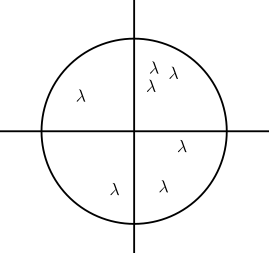
\includegraphics[scale=0.55]{img/th_hirch.png}
\end{figure}

Ossia ogni autovalore deve essere inferiore alla norma matriciale indotta.
E' come se stessimo "localizzando" la posizione degli autovalori.

\paragraph{Dimostrazione} Dimostriamo il teorema:

\begin{enumerate}
    \item Dalla definizione di autovalore:
    \[ A\:v = \lambda\:v \:\:\: \text{con} \:\:\: \lambda \neq0\]
    \item Applico la norma a sx e dx ed inverto l'ordine:
    \[ ||\:\lambda\:v\:|| = ||\:A\:v\:||\]
    \item Proprietà $(2.)$ e $(4.)$ delle norme matriciali:
    \[ |\lambda|\:||\:v\:|| = ||\:A\:v \:|| \leq ||\:A\:|| \:||\:v\:|| \]
    \item Considero dunque primo e terzo termine, dividendo a sx e dx per $||v||$:
    \[ \boxed{|\lambda| \leq ||A||} \]
\end{enumerate}

\newpage

\subsection{Utilities Greshgorin}

Elenchiamo tutte gli oggetti e funzioni definiti sui cerchi di Gershgorin:

\subsubsection{Cerchio i-esimo di Greshgorin}

Definiamo un cerchio come luogo geometrico dei punti, dato che successivamente sarà necessario alla localizzazione degli autovalori.

\paragraph{Definizione} Sia $K_{i}$ dove
\[ \boxed{K_{i} = \{ z \in \mathbb{C} \: : \: |z-a_{ii}| \leq \sum_{j=1, j\neq i}^{n}|a_{ij}|  \: \} }\]

\begin{enumerate}
    \item $a_{ii}$ corrisponde al \textbf{centro} del cerchio.
    \item $\sum_{j=1, j\neq i}^{n}|a_{ij}|$ corrisponde al \textbf{raggio} del cerchio.
\end{enumerate}

\subsubsection{Th. di Greshgorin (con Dim.)}

Il teorema di Greshgorin afferma che se un arbitrario $\lambda$ è un autovalore, allora questo deve essere all'interno dell'unione dei cerchi di Greshgorin della matrice.

\paragraph{Definizione} $\boxed{\text{Se} \: \: \: \lambda \: \: \: \text{è} \: \: \: \textbf{autovalore} \: \: \: \text{di} \: \: \: A \: \:\Rightarrow \: \: \lambda \in \bigcup_{i=1}^{n}k_{i}} $

\vspace*{12px}

Spesso questo teorema viene utilizzato "al contrario", ossia se un valore \textbf{non} è all'interno dell'unione dei cerchi, allora sicuramente \textbf{non} è un autovalore della matrice.

\paragraph{Dimostrazione} Dimostriamo il teorema:

\begin{enumerate}
    \item Dalla definizione di autovalore:
    \[ A\:v = \lambda \: v \]
   \[ \begin{bmatrix}
    a_{11} & a_{12} & ... & a_{1n}\\
    a_{21} & a_{22} & ... & a_{2n}\\
    . & . & . & . \\
    a_{n1} & a_{n2} & ... & a_{nn}
    \end{bmatrix} 
    \begin{bmatrix}
        v_1 \\
        v_2 \\
        . \\
        v_n \\
    \end{bmatrix} \: = \: \lambda 
    \begin{bmatrix}
        v_1 \\
        v_2 \\
        . \\
        v_n \\
    \end{bmatrix} \]
    \vspace*{5px}
    \item Assumo di aver effettuato il prodotto ad sx tra $A$ e $v$:
    \[ \sum_{j=1}^{n} a_{ij}v_{j} = \lambda v_{i} \:\:\:\: \forall \: i \in \{ 1\:,... ,\:n \}  \]
    \item Tiro fuori dalla sommatoria il termine per $i=j$, lo porto a sinistra e metto in evidenza $v_{i}$:
    \[ \sum_{j=1,j\neq i}^{n} (a_{ij}v_{j})  = (\lambda - a_{ii} )v_{i} \]
    \newpage
    \item Sapendo che:
    \[ \boxed{|\lambda-a_{ii}|\:|v_{i}|  =  | (\lambda - a_{ii})v_{i} |} \:\:\: \text{e} \:\:\: \boxed{|\sum_{j=1}^{n} a_{ij}v_{j} \:  | \leq \sum_{j=1}^{n} \:|a_{ij}|\:|v_{j}|} \]
    \item Prendo un $p$ tale che:
    \[ 0 \leq |v\:p| = ||v|| = max_{j=1..n} \: |v_{j}| \]
    Ossia $p$ deve fare in modo che la norma di $v$ deve essere uguale al massimo delle componenti del vettore $v$. Assumiamo di non star lavorando sul vettore nullo grazie alla definizione di autovalore $\lambda$.
    \item Istanzio il punto $(3.)$ con la $p$ appena definita in $(5.)$:
    \[ |\lambda - a_{pp }|  |v_{p}| \leq \sum_{j=1,j \neq i}^{n} |a_{pj}| |v_{j}| \]
    \item Divido a sx e dx per $|v_{p}|$:
    \[ |\lambda - a_{pp }|  \frac{|v_{p}|}{|v_{p}|} \leq \sum_{j=1,j \neq i}^{n} |a_{pj}| \frac{|v_{j}|}{|v_{p}|} \]
    Sappiamo che $\frac{|v_{j}|}{|v_{p}|} \leq 1$ perchè in un vettore possiamo avere più massimi, quindi componenti max con stessi valori.
    \item Riesco dunque ad effettuare una maggiorazione grazie alle affermazioni precedenti:
    \[ \sum_{j=1,j \neq i}^{n} |a_{pj}| \frac{|v_{j}|}{|v_{p}|} \leq \sum_{j=1,j \neq i}^{n} |a_{pj}| \]
    \item La sommatoria ottenuta nella maggiorazione del punto $(8.)$ rispetta la definizione di \textit{Cerchio i-esimo di Gershgorin}, di conseguenza abbiamo dimostrato il teorema. $\boxed{}$
    \[ \boxed{\lambda \in K_{p}} \]
    
\end{enumerate}

\subsubsection{Invertibilità e Predominanza Diagonale}

\paragraph{Matrice Invertibile} Elenchiamo un paio di caratteristiche sull'invertibilità di matrici:

\begin{enumerate}
    \item Se $A$ è invertibile, allora:
    \begin{enumerate}
        \item $det(A) \neq 0 $
        \item $rango(A) = 0$
        \item $dim(ker(A)) = 0$
        \item $0$ non è un autovalore
        \item $P(x) = det(A-xI) = (x-\lambda_{1})(x-\lambda_{2})....(x-\lambda_{n})$
        \item $P(0) = det(A) = (x-\lambda_{1})(x-\lambda_{2})....(x-\lambda_{n}) = \text{ prodotto degli autovalori }\lambda_{i}$
    \end{enumerate}
\end{enumerate}

\paragraph{Predominanza Diagonale di Matrice per Riga} La predominanza vale quando in valore assoluto, l'elemento sulla diagonale principale è maggiore di tutti gli altri sulla riga, formalmente:

\[ |a_{ii}| > \sum_{j=1,j \neq i}^{n}|a_{ij}| \]

\subparagraph{Corollario} Se $A$ è a \textbf{predominanza diagonale} allora $A$ è \textbf{invertibile}. La dimostrazione di questo corollario si basa sul fatto che la definizione appena data si basa sul \textit{Cerchio di Gershgorin} ma utilizzato al contrario, ossia stiamo affermando di \textbf{non} essere nel cerchio. Questo però ci porta ad essere esattamente al contrario rispetto ****.

\subsubsection{II Th. di Gershgorin}

\paragraph{Definizione} Se l'\textbf{unione} $M_{1}$ di $k$ cerchi è \textbf{disgiunta} dall'\textbf{unione} $M_{2}$ di $(n-k)$ cerchi allora $k$ autovalori appartengono ad $M_{1}$ ed $(n-k)$ ad $M_{2}$.

\subsection{Condizionamento del Problema sulla Risoluzione di Sistemi Lineari}

Assumiamo di avere una matrice $A$ ed un vettore $b$, $Ax = b$, sapendo che se $A$ è invertibile allora $x = A^{-1}b$, altrimenti o non ha soluzioni o ne ha infinite. Elenchiamo come approssimeremo questi oggetti in oggetti discreti:

\begin{enumerate}
    \item \textbf{Matrice} $A$ ed i suoi \textbf{elementi} $a_{ij}\:$:
    \[ \tilde{A} = A + \Delta A  \:\:\: \:\:\: \:\:\: \tilde{a}_{ij} = a_{ij} + \epsilon  f_{ij}  \]
    dove $f_{ij} = (1+\epsilon_{ij})$, ossia l'errore su ogni componente, e $\Delta A$ li contiene tutti.
    \item \textbf{Vettore} $b$ ed i suoi \textbf{elementi} $b_{i}\:$:
    \[ \tilde{b} = b + \delta b  \:\:\: \:\:\: \:\:\: \tilde{b}_{i} = b_{i} + (1+f_{i})  \]
\end{enumerate}

Il \textbf{condizionamento} verrà quindi calcolato su \textbf{norme}:

\[ \frac{||\tilde{x}-x||}{||x||} \]

Vogliamo dunque esprimere la risoluzione in questa forma:

\[ x = A^{-1}b \]

\subsubsection{Teorema sul Condizionamento di Norme Matriciali (con dim)} 

\paragraph{Definizione} Sia $A$ invertibile e $b \neq 0$, allora:

\[ \frac{||\tilde{x}-x||}{||x||} \leq ||A||\:\:||A^{-1}|| \frac{||\tilde{b}-b||}{||b||} \]

Dove $||A||\:\:||A^{-1}||$ è detto \textbf{numero di condizionamento} di A.

\newpage

\paragraph{Dimostrazione} Dimostriamo questo teorema:

\begin{enumerate}
    \item Partiamo dalla definizione di $x$ ed $\tilde{x}$:
    \[ x = A^{-1}b \: \:\rightarrow \: \: Ax = b\]
    \[ \tilde{x} = A^{-1}\tilde{b} \: \:\rightarrow \: \: A\tilde{x} = \tilde{b}\]
    \item Sostituiamo $(1.)$ in $||\tilde{x}-x||$:
    \[ || \: A^{-1}\tilde{b} \: - \: A^{-1}{b} \: || \]
    \item Raccolta di $A^{-1}$ e compatibilità di norme a motivazione del $(\leq)$:
    \[ ||\tilde{x} - x|| = ||A^{-1}(\tilde{b}-b)|| \leq ||A^{-1}|| \: \: ||\tilde{b}-b|| \]
    \item Scriviamo la forma standard di risoluzione di sistema lineare applicando le norme a sx e dx, e utilizziamo anche qui la compatibilità delle norme per $(\leq)$ a dx:
    \[ ||Ax|| = ||b|| \: \rightarrow \: ||b|| = ||Ax|| \leq ||A|| \: \: ||x|| \]
    \item Da questo possiamo dunque ricavare che:
    \[ ||x|| \: ||A|| \geq  ||b|| \rightarrow ||x|| \geq \frac{||b||}{||A||} \]
    \item Tornando dunque al punto (3.) possiamo dividere $||\tilde{x} - x||$ per $||x||$ ed a dx del $\leq$ dividiamo per $\frac{||b||}{||A||}$ rispettando quindi la maggiorazione (dato il punto precedente).
    \[ \frac{||\tilde{x}-x||}{||x||} \leq ||A|| \: ||A^{-1}|| \: \frac{||\tilde{b}-b||}{b} \] 
    \item Avendo concluso la dimostrazione definiamo $\mu$, il \textbf{numero di condizionamento} di $A$:
    \[ \mu = ||A||\:||A^{-1}|| \]
\end{enumerate}

\newpage

\section{Metodi Diretti per Risoluzione di Sistemi Lineari}

Assumiamo di avere $Ax = b, \: \: \: A\in \mathbb{R}^{nxn}, \: \: \: det(A)\neq0, \: \: \: x = A^{-1}b$, allora possiamo avere diversi casi:

\begin{enumerate}
    \item \textbf{Matrice Diagonale}: La matrice $A$ ha solo elementi sulla sua diagonale.
    \[ 
    \begin{bmatrix}
    a_{11} & 0 & ...  & 0\\
    0 & a_{22} &  & ...\\
     ...&  & a_{33} &  0\\
     0& ... & 0 & a_{nn}
    \end{bmatrix} 
    \]
    In questo caso possiamo ricavare le \textbf{soluzioni} in questo modo
    \[ x = A^{-1}b = \begin{bmatrix}
    \frac{1}{a_{11}} & 0 & ...  & 0\\
    0 & \frac{1}{a_{22}} &  & ...\\
     ...&  & \frac{1}{a_{33}} &  0\\
     0& ... & 0 & \frac{1}{a_{nn}}
    \end{bmatrix}
    \begin{bmatrix}
    b_{1}\\    
    b_{2}\\
    b_{3}\\
    b_{n}
    \end{bmatrix}  \]
    Ricordiamo che il costo di questa risoluzione risulta essere $O(n)$.
    \item \textbf{Matrice Triangolare}: La matrice $A$ è diagonale e di conseguenza gli \textit{autovalori} sono gli elementi sulla diagonale. Dunque possiamo calcolare il determinante in questo modo:
    \vspace*{10px}
    \[
    \begin{bmatrix}
    a_{11} & ... & ...  & a_{1n}\\
    0 & a_{22} &  & ...\\
     ...&  & a_{33} &  ...\\
     0 & ... & 0 & a_{nn}
    \end{bmatrix}
    \]
    \vspace*{5px}
    \[ det(A) = \prod_{i=1}^{n} a_{ii} \]
    \vspace*{5px}
    In questo caso le \textbf{soluzioni} si ottengono grazie al \textbf{metodo di sostituzione}. (Il metodo di sostituizione in avanti o in indietro in base a se la matrice risulta triangolare superiore o inferiore). Il costo di questa risoluzione risulta essere $O(n^{2})$.
    \item \textbf{Matrice Piena}: La matrice $A$ risulta piena:
    \[
    \begin{bmatrix}
    a_{11} & ... & ...  & a_{1n}\\
    ... & a_{22} &  & ...\\
     ...&  & a_{33} &  ...\\
     a_{n1} & ... & ... & a_{nn}
    \end{bmatrix}
    \]

    Non si conosce un algoritmo che sia aderente al limite inferiore $O(n^{2})$ del problema. Di conseguenza l'algoritmo favorito in queste circostanze è quello di \textbf{Gauss}, caratterizzato da un costo in tempo asintotico $O(n^{3})$, dato che bisogna, per ogni colonna, azzerare tutti gli elementi sotto la diagonale.
    
\end{enumerate}

\newpage

\subsection{Fattorizzazione LU}

Grazie al Th. di Gauss riusciamo ad ottenere anche una nuova \textbf{formulazione} di matrici piene sotto specifiche ipotesi.

\paragraph{Definizione di Fattorizzabile} Una matrice $A \in \mathbb{R}^{nxn}$ è \textit{fattorizzabile LU} se

\begin{enumerate}
    \item Esiste $L$ matrice triangolare inferiore con elementi diagonali uguali ad $1$.
    \item Esiste $U$ matrice triangolare superiore.
\end{enumerate}

Tale che

\vspace*{-8px}

\[ \boxed{A = LU} \]

\subsection{Th. Condizioni Sufficienti per Esistenza ed Unicità Fattorizzazione LU (con Dim.)}

Assumiamo di avere una matrice quadrata $A \in \mathbb{R}^{nxn}$, definiamo con $A_{k}$ le sue sottomatrici quadrate di dimensione $k \: * \: k$. Questo darà contesto alla definizione formale del teorema.

\paragraph{Definizione} Sia $A \in \mathbb{R}^{nxn}$ se $det(A_{k}) \neq 0 \: \: \: \forall k \in \{ 1,\:...,\:n-1 \}$ allora esiste la \textit{fattorizzazione LU} di $A$.

\paragraph{Dimostrazione}

Procediamo a dimostrare per induzione questo teorema:

\begin{enumerate}
    \item \textbf{Caso Base}: Prendiamo $k=1$, quindi $A=\begin{bmatrix}
       a_{11}
   \end{bmatrix}$ dunque:
   \[ L=\begin{bmatrix}
       1
   \end{bmatrix} \: \: \:
   U=
   \begin{bmatrix}
       a_{11}
   \end{bmatrix} \:\:\:
   \text{allora}
   \:\:\:
   A=LU\]
   \item \textbf{Caso Induttivo}: Assumiamo che la proprietà sia vera sulle matrici di dimensione $n-1$ (Ipotesi Induttiva).
   \begin{enumerate}
       \item Vediamo le matrici $A, L, U$ a blocchi rispettivamente in questo modo:
       \[ \begin{bmatrix}
           A_{n-1} & | & x\\
           \hline
           y^T & | & a_{nn}
       \end{bmatrix} =
       \begin{bmatrix}
           L_{n-1} & | & 0\\
           \hline
           w & | & 1
       \end{bmatrix}
       \begin{bmatrix}
           U_{n-1} & | & z\\
           \hline
           0^T & | & \beta
       \end{bmatrix}
       \]
       \item Consideriamo ogni elemento della matrice $A$ come prodotto dei blocchi delle matrici $L$ ed $U$:
       \begin{enumerate}
           \item Prodotto prima riga di $L$ prima colonna di $U$:
           \[ A_{n-1} = L_{n-1}U_{n-1} + 0\:0^{T}\]
           Rimuovendo gli zeri, otteniamo questo primo blocco di $A$ valido per ipotesi induttiva.
           \newpage
           \item Prodotto prima riga di $L$ seconda colonna di $U$:
           \[ x = L_{(n-1)}z + 0 \: \beta  \]
           La matrice $L_{(n-1)}$ è valida per ipotesi induttiva, esisterà almeno una $z$ per cui $z=L^{-1}_{n-1}x$.
           \item Prodotto seconda riga di $L$ prima colonna di $U$:
           \[ y^{T} = w^{T}U_{n-1} + 1\:0^{T} \]
           Trasponendo otteniamo:
           \[ y = U^{T}_{n-1}w \]
           \item Prodotto seconda riga di $L$ seconda colonna di $U$:
           \[ a_{nn} = w^{T}z + 1\beta \]
       \end{enumerate}
   \end{enumerate}
\end{enumerate}

\subsection{Matrici Elementari di Gauss}

Definiamo la matrice $E$:

\[ E = I -ve^{T}_{k} \:\:\: \text{con} \:\:\: e_{k} = \begin{bmatrix}
    0 \\
    . \\
    0 \\
    1 \\
    0 \\
    . \\
    0 \\
    
\end{bmatrix}
\:\:\: \text{e} \:\:\: 
v_{1} = v_{2} = v_{k}
\]

$E$ è quindi definita come \textbf{Matrice di Gauss}.

\paragraph{Proprietà} Questo tipo di matrice gode di diverse proprietà caratteristiche:

\begin{enumerate}
    \item Queste matrici sono \textbf{triangolari inferiori} con tutti $1$ sulla diagonale e sono \textbf{invertibili}.
    \item Vale che:
    \vspace*{5px}
    \[ E^{-1} = I + ve^T_k \]
    \vspace*{5px}
    Questo statement si può dimostrare effettuando la moltiplicazione tra $E$ ed $E^{-1}$ ottenendo $I$.
    \item Sia $x \in \mathbb{R}^{n}$ con $x_{k} \neq 0$. Allora esiste una matrice elementare di Gauss tale che
    \[ Ex = {\begin{bmatrix}
        x_{1} & ... & x_{k} & 0 & ... & 0
    \end{bmatrix}}^{T} \]
    \newpage
    \item Assumendo di avere due matrici elementari di Gauss:
    \[ \boxed{E = I - ve^T_k} \:\:\:\:\:\: \boxed{\overline{E} = I - we^T_l} \]
    allora
    \[ \boxed{E \: \overline{E} = I_{n} - ve_{k}^{T} - we_{l}} \]
    che informalmente vuol dire che il prodotto tra le due matrici elementari di Gauss viene costruito posizionando
    semplicemente nella posizione corretta i due vettori $v$ e $w$ di fattori.
    \item Il prodotto di $Ey$, dove $E = I - ve_{k}^{T}$ è una matrice elementare di Gauss ed $y$ un vettore, può essere calcolato in $n-k$
    operazioni moltiplicative, infatti ponendo $Ey = z$ otteniamo che $z_{j} = y_{j}$ per $1 \leq j \leq k$ mentre $z_{j} = y_{j} - v_{j}y_{k}$.
\end{enumerate}

\vspace*{10px}

Il metodo di Gauss può essere utilizzato senza scambio di \newline righe se e solo se
$a^{k-1}_{kk} \neq 0 \:\:\: \forall k = 1 \: ... \: n$, ossia se tutti i pivot risultano essere diversi da 0.

\paragraph{Teorema} Dato un $A \in \mathbb{R}$: 

\[ A(1:k,1:k) \neq 0  \Leftrightarrow p^{k-1}_{kk} \neq 0 \:\: \forall k \in \{ 1, \: ... \:, n-1  \} \]

E quindi, considerando che $Ly = b$:

\[ [A|B] \: \rightarrow_{E_{1}} \:\: ... \:\: \rightarrow_{E_{2}} \:\: ... \:\: \rightarrow_{E_{n-1}} = [U|y] \] 

\subsection{Tecniche di Pivoting}

Assumiamo di avere un pivot pari a $0$, è necessario che si generi una \textbf{permutazione}
della corrente matrice per fare in modo che il pivot in questione non sia nullo.
\[
    \begin{bmatrix}
    a_{11} & * & *  & * \\
    0 & 0_{k+1} &  & ...\\
     ...& ... & ... &  ...\\
     0 & a_{nk} & 0 & *
    \end{bmatrix}
\]

Questo mi causa però la \textbf{fattorizzazione LU} di una permutazione della matrice
$A$ e non di $A$ stessa.

\[ U = E_{n-1}P^{n-1} \:\:\: ... \:\:\: E_{(1)}P^{(1)}E_{(0)}P^{(0)}A^{(0)} \]

\paragraph{Stabilità e Pivoting} Le tecniche di pivoting non sono utilizzate solo
nel caso in cui un pivot risulti nullo, ma anche per questioni di stabilità degli
algoritmi causati.

Si può dunque dimostrare che i fattori $\tilde{L}$ e $\tilde{U}$ calcolati sono tali
per cui $\tilde{L} \tilde{U} = A + E $, dove $E$ corrisponde all'errore in rappresentazione
in numeri di macchina.
Vale dunque che:

\[ \frac{||E||}{||\tilde{L}||\:\: ||\tilde{U}||} = O(u) \]

\newpage

\section{Metodi Iterativi per Risoluzione di Sistemi Lineari}

Perchè abbiamo la necessità di nuovi metodi oltre a quello di Gauss? Immaginiamo di avere questa matrice (ad albero):

\[
\begin{bmatrix}
    1 & ... & ... & 1\\
    . & .   & 0 & 0 \\
    . & 0 & .& 0 \\
    1 & & & 1
\end{bmatrix}
\]

Applicare qui Gauss causerebbe il fenomeno del \textbf{fill-in}, aumentando il costo. L'idea sarebbe quella di approssimare $Ax = b$ grazie a questi passi:

\begin{enumerate}
    \item $x^{(0)}$ è il vettore iniziale.
    \item $\{ x^{(k)} \}$ è una successione di vettori.
    \item Con approssimazione si intende quindi che il limite all'infinito di ogni componente deve corrispondere a:
    \[ \lim_{k \rightarrow \infty} x^{(k)} = x \Leftrightarrow \lim_{k \rightarrow \infty} x^{(k)} - x \Leftrightarrow \lim_{k \rightarrow \infty} ||\:x^{(k)} - x \:|| = 0 \]
    Con questo riusciamo a dare una prima definizione alla convergenza di successione definita prima.
\end{enumerate}

\paragraph{Criterio d'Arresto} Non vado effettivamente all'infinito ma scelgo un numero di passi $k$ discreto che mi stabilisce il numero di volte che reitererò il metodo. Elenchiamo qualche criterio utilizzabile:

\begin{enumerate}
    \item Un numero $k$ completamente arbitrario.
    \item $||\: x^{(k+1)} - x^{(k)} \:|| \leq \text{tolleranza} \approx 10^{-8} \:\: \text{oppure} \:\: 10^{-12} $
    \item $||\: Ax^{k} - b \:|| \leq \text{tolleranza}$
\end{enumerate}

Nessuno di questi garantisce che l'errore generato sarà $<$ della tolleranza.

\subsection{Metodi Basati sulla Decomposizione Additiva}

Data $Ax = b$, assumiamo che $A = M - N$ con $M$ invertibile. Sostituiamo l'assunzione nella definizione originale:

\vspace*{8px}

\begin{enumerate}
    \item Sostituzione:
    \[ (M - N)x = b \Leftrightarrow Mx - Nx = b \Leftrightarrow Mx = Nx + b  \]
    \vspace*{15px}
    \item Dato che $M$ invertibile per ipotesi allora moltiplichiamo sx e dx per $M^{-1}$:
    \[ x = M^{-1}Nx + M^{-1}b \]
    \item Ponendo $P=M^{-1}N$ matrice di iterazioni e $p = M^{-1}b$, allora $x = Px + q$, quindi al passo k-esimo:
    \vspace*{8px}
    \[ x^{k+1} = Px^{(k)} + q \:\:\:\: \text{con} \:\: x^{(0)} \in \mathbb{R}^{n} \]
    \item Quindi la \textbf{successione} è detta \textbf{convergente} se:
    \[ \lim_{k \rightarrow \infty} ||\: x^{(k)} - x \:|| = 0 \]
    \item Il \textbf{metodo} $(P,q)$ è detto \textbf{convergente} invece se: 
    \[ \forall \: x^{(0)} \Rightarrow \:\: \text{la successione} \:\: \{ x^{(k)} \} \:\: \text{è convergente}\]
\end{enumerate}

\subsection{Th. Condizioni Sufficienti per la Convergenza di Metodo (con Dim.)}

Definiamo il teorema:
%possiamo fixare graficamente la funzione definita nella tesi, per ora si lascia così

\begin{enumerate}
    \item \textbf{Ipotesi}: Se esiste una norma matriciale indotta in cui $||P|| < 1$, allora:
    \item \textbf{Tesi}: Il metodo definito sotto converge.
    \vspace*{10px}
    \[ \left\{ \begin{array}{rcl}
        x^{(0)} \in \mathbb{R}^{n} \\ 
        x^{k+1} = Px^{(k+1)} + q 
        \end{array}\right.
         \]
\end{enumerate}

\paragraph{Dimostrazione} Dimostriamo il teorema per step:

\begin{enumerate}
    \item Prendo la successione:
    \[ x^{(k+1)} = Px^{(k)} + q \]
    e voglio che questa converga ad $x=Px+q$, ossia che la distanza tra $x^{(k)}$ ed $x$ tende a $0$ per $x \rightarrow +\infty$.
    \vspace*{15px}
    \item Consideriamo $e^{(k)}$ vettore errore alla k-esima iterazione:
    \[ e^{(k)} = x^{(k)} - x  \Leftrightarrow \]
    \[ \Leftrightarrow e^{(k+1)} = x^{(k+1)} - x \]
    \vspace*{15px}
    \item Sostituiamo le definizioni di $x^{(k+1)}$ e $x^{(k)}$ date in $(1.)$ in $e^{(k+1)}$ data in $(2.)\:$:
    \[ e^{(k+1)} = Px^{(k)} + q - (Px+q) = Px^{(k)} - Px = Pe^{(k)} \]
    \vspace*{15px}
    Vogliamo dunque impostare induzione su $\boxed{e^{(k+1)} = P^{(k+1)}e^{(0)}}$.
    \newpage
    \item Dimostrazione induttiva:
    \begin{enumerate}
        \item \textbf{Caso Base}: $k=0$, allora $e^{(1)} = Px^{(0)} + q - Px - q = Pe^{(0)}$ 
        \item \textbf{Ipotesi Induttiva}: $ \boxed{e^{(k)} = P^{k}e^{(0)}} $
        \item \textbf{Caso Induttivo}: Lavoriamo sull'n-esimo passo:
        \[ e^{(k+1)} = Pe^{(k)} = P \: P^{k} e^{(0)} = P^{(k+1)} e^{(0)} \Rightarrow e^{(k+1)} = P^{(k+1)}e^{(0)} \]
        Una volta raggiunto questo punto, rielaboro questa espressione grazie alle norme:
    \end{enumerate}
    \item Utilizziamo proprietà norme (vettoriale che induce matriciale, come chiedono le ipotesi del teorema), nello specifico la compatibilità:
    \[ ||\: e^{(k+1)} \:|| = ||\: P^{(k+1)} e^{(0)} \:|| \leq ||\: P^{(k+1)} \:|| \: ||\: e^{(0)} \:|| \]
    \item Possiamo tirare fuori l'esponente dato che $P^{(k+1)} = P\:^{(k)} $, quindi 
    \[ ||\: P \: P^{(k)} \:|| \leq ||P|| \:\: ||P^{(k)}|| \]
    Grazie a questo possiamo dire che
    \[ ||\: e^{(k+1)} \:|| \leq ||\: P^{(k+1)} \:|| \: ||\: e^{(0)} \:|| \leq ||\: P \:||^{(k+1)} \: ||\: e^{(0)} \:||\]
    Sappiamo anche che $||\: P \:||^{(k+1)} \: ||\: e^{(0)} \:|| = 0$ dato che $0 < ||\:P\:|| < 1 $.
    \item Per il teorema del confronto quindi:
    \[ \lim_{k \rightarrow \infty} ||\: e^{(k+1)} \:|| = 0 \Longleftrightarrow \lim_{k \rightarrow \infty} e^{(k)} \Longleftrightarrow \lim_{k \rightarrow \infty} x^{(k)} = x \:\:\: \boxed{} \] 
\end{enumerate}

\subsection{Th. Condizioni Necessarie per la Convergenza di Metodo (con Dim.)}

Definiamo il teorema:
%possiamo fixare graficamente la funzione definita nella tesi, per ora si lascia così

\begin{enumerate}
    \item \textbf{Ipotesi}: Se il metodo definito sotto è convergente, allora:
    \item \textbf{Tesi}: Il raggio spettrale $\rho(P) < 1$.
    \vspace*{10px}
    \[ M = \left\{ \begin{array}{rcl}
        x^{(0)} \in \mathbb{R}^{n} \\ 
        x^{k+1} = Px^{(k+1)} + q 
        \end{array}\right.
         \]
\end{enumerate}

Dimostriamo il teorema a pagina successiva.

\newpage

\paragraph{Dimostrazione} Dimostriamo il teorema per step:

\begin{enumerate}
    \item Per ipotesi (convergenza) sappiamo che:
    \[ e^{(0)} = x^{(k)} - x^{(0)} = P^{(k)}e^{(0)} \:\: \text{e tale che} \:\: \forall \: x^{(0)} \: \: \lim_{k \rightarrow \infty} e^{(k)} = 0\]
    \item Sapendo che il metodo converge per ogni successione da ipotesi allora ne scelgo una particolare, in modo tale da far apparire il raggio spettrale:
    \[ x^{(0)} = x + v \]
    dove
    \begin{enumerate}
        \item $x = Px + q$ corrisponde alla soluzione.
        \item $v$ è l'autovettore con autovalori di $P$, ossia $|\lambda| = \rho(P)$.
    \end{enumerate}
    \item Possiamo dunque tornare alla definizione data in $(1.)$ inserendo la definizione appena data in $(2.)$:
    \[ e^{(k)} = P^{(k)}e^{(0)} = P^{(k)}(x^{(0)} - x) = P^{(k)}v = \lambda^{(k)}v \]
    \item Grazie al limite dato in $(1.)$ ed ad il primo e l'ultimo termine di $(3.)$:
    \[ 0 = \lim_{k \rightarrow \infty} ||\:e^{(k)}\:|| = \lim_{k \rightarrow \infty} ||\:\lambda^{(k)} \: v \:|| = \lim_{k \rightarrow \infty} ||\:\lambda^{(k)} \:||\:\:||\: v \:|| = \]
    Dato che $v$ è un autovettore sicuramente $||v|| \neq 0$ e il tutto dipenderà dunque da $|\lambda|$:
    \[ = ||v|| \lim_{k \rightarrow \infty} |\lambda^{(k)}| \]
\end{enumerate}

\subsection{Th. Condizione Necessaria e Sufficiente per la Convergenza di Metodo (con Dim.)}

\vspace*{12px}

\[ \text{Un metodo iterativo} \: M = \left\{ \begin{array}{rcl}
    x^{(0)} \in \mathbb{R}^{n} \\ 
    x^{k+1} = Px^{(k+1)} + q 
    \end{array}\right.
    \: \text{è convergente} \:
    \Longleftrightarrow
    \:
    \rho(P) < 1
    \]

\paragraph{Dimostrazione} Dimostriamo il teorema per step, entrambi i versi d'implicazione:

\begin{enumerate}
    \item \textbf{Implicazione Destra}: Condizioni necessarie dimostrate con il teorema precedente.
    \item \textbf{Implicazione Sinistra}: Solo se $P$ è diagonalizzabile:
    \begin{enumerate}
        \item Se $P$ è diagonalizzabile e $\rho(P) < 1 \Rightarrow$ il metodo converge. Ma essendo diagonalizzabile:
        \[ \exists \: S \:\:\: \text{invertibile tale che} \:\:\: P = SDS^{-1} \:\: \text{dove} \:\: D = \begin{bmatrix}
            \lambda_{1} & & & \\
            & \lambda_{1} & & \\
            & & . & \\
            & & & \lambda_{n}
        \end{bmatrix} \]
        \newpage
        \item Vogliamo che il vettore dell errore $e_{k}$ tenda a $0$:
        \[ \boxed{e^{(k)} = P^{(k)}e^{(0)}} \]
        \[ e^{(k)} = P^{(k)}e^{(0)} = (SDS^{-1})^{k} \: e^{(0)} = \]
        \[ SDS^{-1}\: SDS^{-1} \: ... \: SDS^{-1} \: e^{(0)} = SD^{k}S\:e^{(0)} \]
        \item Applichiamo lo stesso limite del teorema precedente e le norme agli estremi dell'espressione generata al punto precedente:
        \[ \lim_{k \rightarrow \infty} ||\:e^{(k)}\:|| = \lim_{k \rightarrow \infty} ||\:SD^{k}S^{-1}\:e^{(0)}\:|| \leq \]
        \item Maggiorazione grazie alle proprietà delle norme:
        \[ \leq ||\:S\:||\:||\:S^{-1}\:||\:||\:e^{(0)}\:||\: \lim_{k \rightarrow \infty} ||\:D^{k}\:|| \]
        Dunque se tutti i $\lambda$ di $D^{k} = \begin{bmatrix}
            \lambda_{1} & & & \\
            & \ddots & & \\
            & & \ddots & \\
            & & & \lambda_{n}
        \end{bmatrix} 
        $ se sono tutti $< 1$ allora per $k \rightarrow \infty$ convergono tutti i $\lambda$.
    \end{enumerate}
\end{enumerate}

\subsection{Th. Fa la Cosa Giusta (con Dim.)}

Se $\{ x^{(k)} \rightarrow x^{*} \}$ con $x^{(k+1)} = Px^{(k)} + q \Rightarrow x^{*} = Px^{*} + q$.

\paragraph{Dimostrazione} Dimostriamo il teorema per step:

\begin{enumerate}
    \item $x^{*} = \lim_{k \rightarrow \infty} x^{(k+1)}$
    \item Sostituendo definizione di $x^{(k+1)}$:
    \[ x^{*} = (\lim_{k \rightarrow \infty} Px^{(k)}) + q \]
    \item Essendo continua tiro fuori $P$ dal limite:
    \[ x^{*} = P(\lim_{k \rightarrow \infty} x^{(k)}) + q = Px^{*} + q \:\: \boxed{} \]
\end{enumerate}
\vspace*{-20px}

\paragraph{Interpretazione} Con questo teorema riusciamo dunque ad affermare che se un metodo converge, allora converge
esattamente alla soluzione, appunto fa la cosa giusta.

\vspace*{-10px}

\paragraph{Piccolo Recap Pre-Metodi Iterativi}: Ricapitolando cosa visto fino ad ora, dato un sistema $Ax = b$, grazie ad una operazione di \textbf{splitting}
scriviamo $A = M - N$ con $M$ invertibile, di conseguenza $det(M) \neq 0$. Riscrivendola abbiamo $(M-N)x = b \Leftrightarrow $ \\ $Mx = Nx + b \Leftrightarrow X = Px + q$ dove $P$ è
la matrice di iterazione ed è definita \\ come $P = M^{-1}\:N$. Se non riuscissi a trovare una norma tale per cui $||P|| > 1$ allora non potrei affermare nulla sulla convergenza dei metodi. 
Questo recap sarà utile durante l'introduzione dei due metodi iterativi presentati a pagina successiva.

\newpage

\subsection{Metodi Iterativi - Jacobi/Gauss-Seidel}

Presentiamo due metodi di decomposizione additiva basati sulla scelta della matrice $M$ ed $N$ in due diversi modi:

\[ \boxed{A = M - N} \]

Entrambi i metodi richiedono che la matrice $M$ sia invertibile per essere applicati.

\begin{enumerate}
    \item \textbf{Metodo di Jacobi}:
    \[
        M =
        \begin{bmatrix}
        a_{11} & 0 & \cdots & 0 \\
        0 & \ddots &  & \vdots \\
        \vdots &  & \ddots & 0 \\
        0 & \cdots & 0 & a_{nn}
        \end{bmatrix},
        \quad
        N =
        \begin{bmatrix}
        0 & -a_{12} & \cdots & -a_{1n} \\
        -a_{21} & \ddots & \ddots & -a_{2n} \\
        \vdots & \ddots & \ddots & -a_{n-1,n} \\
        -a_{n1} & \cdots & -a_{n,n-1} & 0
        \end{bmatrix}
    \]
    Si sceglie come $M$ la \textbf{diagonale} di $A$, dunque $N$ sarà composta da tutti gli altri elementi negati.
    \item \textbf{Metodo di Gauss-Seidel}:
    \[
        M =
        \begin{bmatrix}
        a_{11} & 0 & \cdots & 0 \\
        a_{21} & \ddots &  & \vdots \\
        \vdots &  & \ddots & 0 \\
        a_{n1} & \cdots & a_{n,n-1} & a_{nn}
        \end{bmatrix},
        \quad
        N =
        \begin{bmatrix}
        0 & -a_{12} & \cdots & -a_{1n} \\
        0 & \ddots & \ddots & -a_{2n} \\
        \vdots & \ddots & \ddots & -a_{n-1,n} \\
        0 & \cdots & 0 & 0
    \end{bmatrix}
    \]
    Si sceglie come $M$ la matrice \textbf{triangolare inferiore} di $A$, dunque $N$ sarà composta da tutti gli altri elementi negati.
    
\end{enumerate}
    \subsubsection{Formulazione Metodo di Jacobi}
    \begin{enumerate}
        \item Riprendiamo la definizione vista nel recap della pagina precedente:
        \[ x = M^{-1}(Nx^{(k)} + b) \Leftrightarrow \]
        \vspace*{-12px}
        \[ \Leftrightarrow Mx = (Nx^{(k)} + b)  = \]
        \item Riscriviamo dunque tutto rispettando i formati di ciascun identificatore:
        \vspace*{8px}
        \[  \begin{bmatrix}
            a_{11} & 0 & \cdots & 0 \\
            0 & \ddots &  & \vdots \\
            \vdots &  & \ddots & 0 \\
            0 & \cdots & 0 & a_{nn}
            \end{bmatrix}
            \begin{bmatrix}
                x^{(k+1)}_{1} \\
                \vdots \\
                \vdots \\
                x^{(k+1)}_{n} 
            \end{bmatrix} 
            =
            \begin{bmatrix}
                b_{1} \\
                \vdots \\
                \vdots \\
                b_{n} 
            \end{bmatrix}
            -
            \begin{bmatrix}
                0 & a_{12} & \cdots & a_{1n} \\
                a_{21} & \ddots & \ddots & a_{2n} \\
                \vdots & \ddots & \ddots & a_{n-1,n} \\
                a_{n1} & \cdots & a_{n,n-1} & 0
            \end{bmatrix}
            \begin{bmatrix}
                x^{(k)}_{1} \\
                \vdots \\
                \vdots \\
                x^{(k)}_{n} 
            \end{bmatrix}
        \]
        \item Consideriamo l'i-esima riga in modo tale da parametrizzare:
        \[ a_{ii}x^{(k+1)}_{i} = b_{i} - ( a_{i1}x^{(k)}_{1} + a_{i2}x^{(k)}_{1} + \cdots + a_{i,i-1}x^{(k)}_{i-1} + a_{i,i+1}x^{(k)}_{i+1} + \cdots
        + a_{in}x^{(k)}_{n} ) \]

        \newpage

        \item Generalizzo ulteriormente utilizzando sommatorie:
        
        \[ x_{i} = \frac{1}{a_{ii}} \left[ b_{i} - \sum_{j=1}^{i-1} a_{ij}x^{(k)}_{j} - \sum_{j=i+1}^{n} a_{ij}x^{(k)}_{j} \right] \]
        \vspace*{3px}
        \item Possiamo dunque ottenere delle stime sui costi in tempo ossia $O(n)$ per ciascuna componente, complessivamente il costo per iterazione sarà $O(n^{2})$.
    \end{enumerate}

\subsubsection{Formulazione Metodo di Gauss-Seidel}

\begin{enumerate}
    \item Riprendiamo la definizione vista nel recap della pagina precedente:
        \[ x = M^{-1}(Nx^{(k)} + b) \Leftrightarrow \]
        \vspace*{-12px}
        \[ \Leftrightarrow Mx = (Nx^{(k)} + b)  = \]
        \item Riscriviamo dunque tutto rispettando i formati di ciascun identificatore:
        \vspace*{8px}
        \[  \begin{bmatrix}
            a_{11} & 0 & \cdots & 0 \\
            a_{21} & \ddots &  & \vdots \\
            \vdots &  & \ddots & 0 \\
            a_{n1} & \cdots & a_{n,n-1} & a_{nn}
            \end{bmatrix}
            \begin{bmatrix}
                x^{(k+1)}_{1} \\
                \vdots \\
                \vdots \\
                x^{(k+1)}_{n} 
            \end{bmatrix} 
            =
            \begin{bmatrix}
                b_{1} \\
                \vdots \\
                \vdots \\
                b_{n} 
            \end{bmatrix}
            -
            \begin{bmatrix}
                0 & a_{12} & \cdots & a_{1n} \\
                0 & \ddots & \ddots & a_{2n} \\
                \vdots & \ddots & \ddots & a_{n-1,n} \\
                0 & \cdots & 0 & 0
            \end{bmatrix}
            \begin{bmatrix}
                x^{(k)}_{1} \\
                \vdots \\
                \vdots \\
                x^{(k)}_{n} 
            \end{bmatrix}
        \]
        \item Consideriamo l'i-esima riga in modo tale da parametrizzare: 
        \[ a_{i1}x^{(k+1)}_{1} = a_{i2}x^{(k+1)}_{2} + \cdots + a_{ii}x^{(k+1)}_{i} = b_{i} - a_{i,i-1}x^{(k)}_{i+1} + a_{i,i-2}x^{(k)}_{i+2} + a_{in}x^{(k)}_{n} \]
        \item Generalizzo ulteriormente utilizzando sommatorie:
        \[ x_{i} = \frac{1}{a_{ii}} \left[ b_{i} - \sum_{j=1}^{i-1} a_{ij}x^{(k+1)}_{j} - \sum_{j=i+1}^{n} a_{ij}x^{(k)}_{j} \right] \]
        \item Anche in questo caso il costo per iterazione sarà $O(n^{2})$.
    
\end{enumerate}

\newpage

\subsubsection{Criterio d'Arresto e Bontà Approssimazione del Metodo Iterativo}

Abbiamo già stabilito quali possono essere dei criteri d'arresto per un metodo iterativo, mostriamone uno:

\[ ||\: x^{(k+1)} - x^{(k)} \:|| \leq tol \]

Torniamo sulla definizione di $x$, $x^{(k)}$ e $x^{(k+1)}$:

\[ \boxed{x = Px + q} \: \: \: \: \: \: \: \: \boxed{x^{(k+1)} = Px^{(k)}+q} \]

Vogliamo dunque identificare un criterio d'arresto anche in base all'errore:

\[ e^{(k)} = x^{(k)} - x^{(0)} \]

Fermarsi secondo un arbitrario criterio d'arresto non implica aver prodotto una buona soluzione perchè la successione potrebbe star convergendo lentamente, producendo così una cattiva approssimazione.
In ogni caso vogliamo definire oggettivamente come valutare un criterio d'arresto:

\begin{enumerate}
    \item Partiamo dal contenuto della norma citata sopra e sottraiamo e sommiamo $x$:
    \[ x^{(k+1)} - x^{(k)} = x^{(k+1)} - x - ( x^{(k)} - x ) = e^{(k+1)} - e^{(k)}\]
    \item Avevamo dimostrato che l'errore al passo $k+1$ era:
    \[ e^{(k+1)} = Pe^{k} \]
    \item Tornando quindi ad $(1.)$ e mettiamo in evidenza $e^{(k)}$:
    \[ Pe^{(k)} - e^{(k)} = e^{(k)}[P - I] \]
    \item Essendo che $e^{(k)} = x^{(k)} - x, \:\:\: e^{(k+1)} = x^{(k+1)} - x$, allora $ Pe^{(k)} - e^{(k)} = (x^{(k+1)} - x^{(k)} )$, possiamo quindi sostituire in $(3.)$:
    \vspace*{10px}
    \[ e^{(k)} = (P - I)^{-1} \: (x^{(k+1)} - x^{(k)} ) \:\:\: \Leftrightarrow \:\:\: \text{(Norme a sx e dx)} \]
    \vspace*{5px}
    \[ || \: e^{(k)} \:|| = ||\: (P - I)^{-1} \: x^{(k+1)} - x^{(k)} \: || \leq \:\:\: \Leftrightarrow \:\:\: \text{(Compatibilità Norme)} \]
    \vspace*{5px}
    \[ \leq ||\: (P - I)^{-1} \: || \: || \: x^{(k+1)} - x^{(k)} \: || \leq \:\:\: \Leftrightarrow \:\:\: ((x^{(k+1)} - x^{(k)}) = tol) \]
    \vspace*{5px}
    \[ \leq ||\: (P - I)^{-1} \: || \: tol \]
    \newpage
    \item Possiamo da questo analizzare la bontà del criterio d'arresto, grazie allo studio 
    
    dell'oggetto $||\: (P - I)^{-1} \: ||$, nello specifico vogliamo analizzare il suo raggio spettrale, ossia il più grande
    in modulo tra gli autovalori:
    \[ \frac{1}{\lambda p - 1} \]
    Questo rapporto è dato dall'inversa della matrice $(P-I)$, di conseguenza un raggio spettrale $\rho(P)$ vicino ad $1$ produrrà una cattiva approssimazione, 
    mentre un raggio spettrale $\rho(P)$ lontano da $1$ produrrà una buona approssimazione.
    

\end{enumerate}

\subsubsection{Th. Condizioni Sufficienti per la Convergenza Metodi Jacobi e Gauss-Seidel (con Dim.)}

Sia $A \in \mathbb{R}$ a predominanza diagonale (riga o colonna), allora:

\begin{enumerate}
    \item $A$ è invertibile.
    \item I metodi di Jacobi e Gauss-Seidel sono applicabili.
    \item I metodi di Jacobi e Gauss-Seidel sono convergenti.
\end{enumerate}

\paragraph{Dimostrazione} Dimostriamo tutte e tre le proprietà elencate sopra:

\begin{enumerate}
    \item Già visto, con i cerchi di Gershgorin ossia:
    \[ |a_{ii}| > \sum_{j=1, j \neq i}^{n} |a_{ij}| \]
    \item Lo dimostriamo utilizzando anche quello che abbiamo appena affermato, ma notando anche che deve essere $\geq 0$:
    \[ |a_{ii}| > \sum_{j=1, j \neq i}^{n} |a_{ij}| \geq 0 \]
    \item Supponiamo per assurdo che i metodi non siano convergenti $\Leftrightarrow \exists \lambda$ tale che $|\lambda| \geq 1$ con $\lambda$ autovalore di $P$ sia di Jacobi sia di Gauss-Seidel:
    \begin{enumerate}
        \item $\lambda$ verifica dunque nell'equazione caratteristica:
        \[ 0 = det(P - \lambda I) = det(M^{-1}N - \lambda I ) = det(M^{-1}N - \lambda (M^{-1}M) ) = \]
        \[ = det(-M^{-1}(\lambda M - N)) = det(-M^{-1}) \: det(\lambda M - N) = 0 \]
        \item Osservando l'ultima espressione del punto precedente, dato che $M$ è invertibile, allora sicuramente dovrà essere l'altro termine della moltiplicazione
        a causare l'uguaglianza con $0$. Di conseguenza:
        \[ \lambda \:\: \text{è autovalore} \Longleftrightarrow H = \lambda M - N \:\: \text{è singolare} \]
\newpage
        \item Bisogna dunque dimostrare che questo è un assurdo dato che $H$ risulta essere a predominanza diagonale. Analizziamo da adesso in poi
        in maniera distinta il comportamento di entrambi i metodi:
        \begin{enumerate}
            \item \textbf{Jacobi}: La matrice $H$ in questo caso corrisponde a:
            \[ H = \begin{bmatrix}
                \lambda a_{11} & a_{ij} & \cdots & a_{ij} \\
                a_{ij} & \ddots & & \vdots \\
                \vdots & & \ddots & a_{ij}\\
                a_{ij} & \cdots & a_{ij} & \lambda a_{nn}
            \end{bmatrix} \]
        Ma questa matrice risulta essere a predominanza diagonale, di conseguenza è un assurdo, formalmente:
        \[ |h_{ii}| = |\lambda a_{ii}| = |\lambda|\:|a_{ii}| \geq |a_{ii}| \geq \sum_{j=1, j \neq i}^{n} |a_{ij}| \]
            \item \textbf{Gauss-Seidel}: La matrice $H$ in questo caso corrisponde a:
            \[ H = \begin{bmatrix}
                \lambda a_{11} & a_{ij} & \cdots & a_{ij} \\
                \lambda a_{21} & \ddots & & \vdots \\
                \vdots & & \ddots & a_{ij}\\
                \lambda a_{n1} & \cdots & \lambda a_{n,n-1} & \lambda a_{nn}
            \end{bmatrix} \]
            Formalmente:
            \[ |\lambda|\:|a_{ii}| = |\lambda| \: \sum_{j=1, j \neq i}^{n} |a_{ij}| = \sum_{j=1}^{i-1} |\lambda| \: |a_{ij}| + \sum_{j=i+1}^{n} |\lambda| \: |a_{ij}| \geq \sum_{j=1}^{i-1} |\lambda a_{ij}| + \sum_{j=i+1}^{n} |a_{ij}| \]
            Quindi $H$ risulta essere a predominanza diagonale, di conseguenza è assurdo.
        \end{enumerate}
    \end{enumerate}
\end{enumerate}

\newpage

\end{document}